% siminos/presentations/kittens/templatt.tex        pdflatex templatt; biber templatt
% $Author: predrag $ $Date: 2021-12-06 16:21:14 -0500 (Mon, 06 Dec 2021) $

% remember to update \date{December 6, 2021}

                        \newif\ifboyscout\boyscouttrue          %% comments     %%
                        \newif\ifsubmission\submissionfalse     %% internal     %%
                        \newif\ifblog\blogfalse %% section shared with blogCats %%

\input ../../inputs/layoutBeamer
\usepackage[font=scriptsize, labelfont=bf]{caption}
\usepackage[
    backend=biber,  %bibtex,
    sorting=nyt,
    %refsection=chapter,
    %citereset=chapter,
    style=numeric, %alphabetic, % %style=authoryear,
    natbib=true,
    style=phys, % aps
    biblabel= brackets, % superscript, %
    articletitle=false, % true,  % false, % aps
    %chaptertitle=true,  % aip;  % false, % aps
    pageranges = true , % aip: the full range
             % = false, % aps: only the first page being printed
    sortlocale=en_US,
    firstinits=true,
    url=false, %true,  %
    doi=false, %true,
    eprint=false
]{biblatex}
\addbibresource{../../bibtex/siminos.bib}
\setbeamerfont{footnote}{size=\tiny}
%\input ../../inputs/def % no edits, always from dasbuch/book/inputs
\input defsKittens
\input ../../inputs/defsBeamer
\renewcommand{\Ssym}[1]{{\ensuremath{m_{#1}}}}    % Boris
% \newcommand{\Ssym}[1]{{\ensuremath{s_{#1}}}}  % ChaosBook
% \newcommand{\D}{\mathcal{D}}
% \newcommand{\gd}{\mathsf{g}}

\begin{document}
\title{
{\huge kicked rotor} %\catlatt}
    \\
{cat in $1$ spacetime dimension}
}
\author{P. Cvitanovi\'c}
\author[Cvitanovi\'c]
{
  \textcolor{green!50!black}{
  {Predrag~Cvitanovi\'c
   and
   Han Liang
%   \\
%  Matt Gudorf,
  }	%\inst{1}
  }
}
\institute
{               Georgia Tech     \\
                {\scriptsize
 ChaosBook.org/overheads/spatiotemporal \\
 $\to$ Chaotic field theory slides    }
 }
\date{December 6, 2021}

%\begin{frame}{} %herding cats}
%\begin{center}
%\hfill
\includegraphics[width=0.95\textheight]{DawnBishopCats}
%\end{center}
%\end{frame} %%%%%%%%%%%%%%%%%%%%%%%%%%%%%%%%%%%%%%%%%%%%%%

\begin{frame}
  \titlepage
\end{frame} %%%%%%%%%%%%%%%%%%%%%%%%%%%%%%%%%%%%%%%%%%%%%%

%\section[what this talk is about]
% {what this talk is about}
%

\begin{frame}{building blocks od turbulence}
\begin{center}
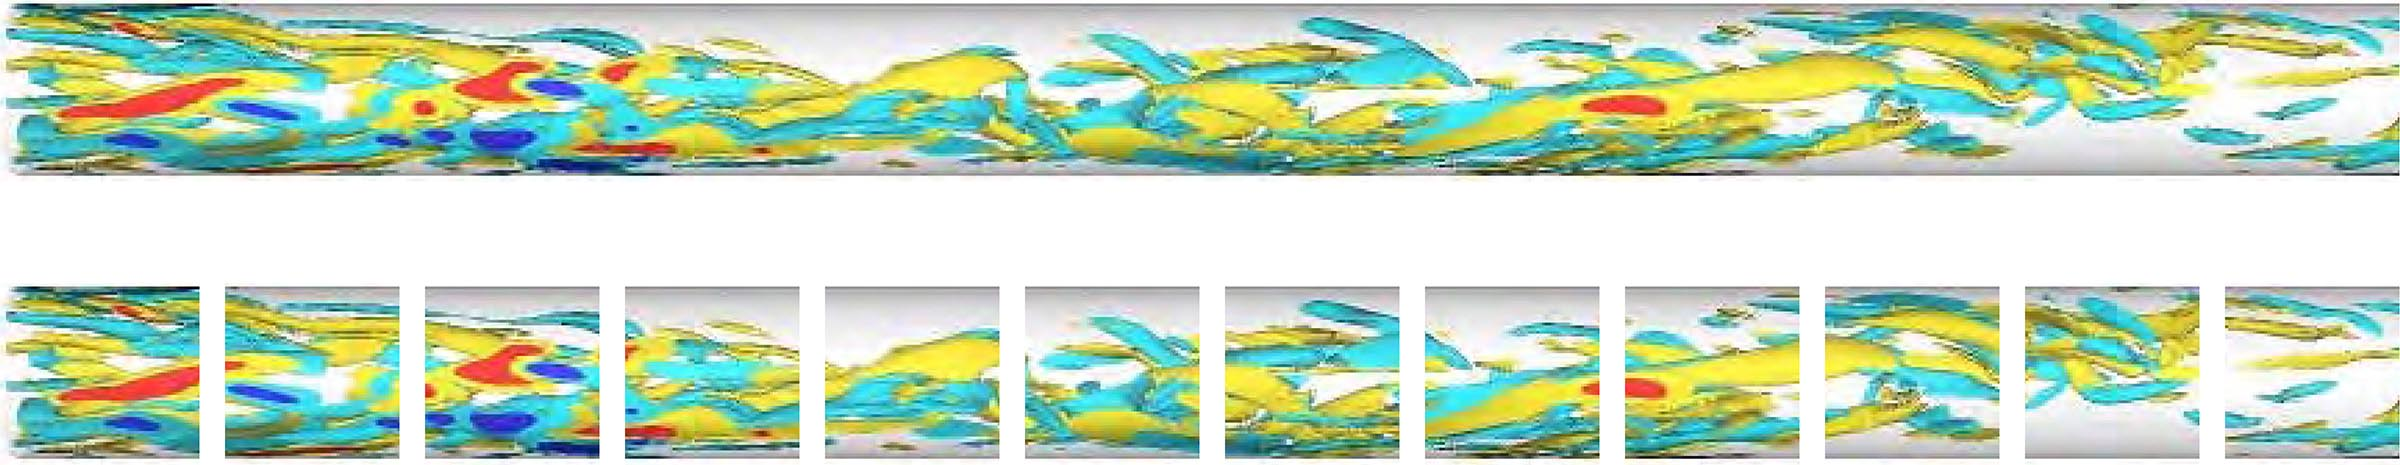
\includegraphics[width=1.0\textwidth]{AviHof13fig4CLM}
\end{center}
have : a detailed theory of {\small \textcolor{blue}{small}} turbulent cells

\bigskip

construct : the \textcolor{red}{infinite} state by coupling turbulent
cells\footfullcite{GuBuCv17}
\vfill

\textcolor{blue}{what would that theory look like ?}
\end{frame} %%%%%%%%%%%%%%%%%%%%%%%%%%%%%%%%%%%%%%%%%%%%%%

\renewcommand{\statesp}{phase space}


\section[a kicked rotor]
 {a kicked rotor}

\begin{frame}{coin toss ? that's not physics !}
Field Theory should be
Hamiltonian and energy conserving \\
Quantum Mechanics requires it

\hfill
because {\color{blue}that is physics} {\color{red}!}
\bigskip

need a system as simple
as the Bernoulli, but {\color{blue}mechanical}
\bigskip

so, we move on from running in circles,

\hfill
to a mechanical {\color{blue}rotor} to kick.
\end{frame} %%%%%%%%%%%%%%%%%%%%%%%%%%%%%%%%%%%%%%%%%%%%%%

\begin{frame}{next : a kicked rotor} % - templatt.tex }
\begin{bartlett}{
Du mu{\ss}t es dreimal sagen!
        }
\bauthor{
Mephistopheles
    }
\end{bartlett}
\vfill
\begin{enumerate}
              \item \textcolor{gray}{\small
\HREF{http://ChaosBook.org/overheads/spatiotemporal/why.pdf}
{what this is about}
              \item
\HREF{http://ChaosBook.org/overheads/spatiotemporal/Bernoulli.pdf}
{coin toss}
                  }
              \item {\Large
\HREF{http://ChaosBook.org/overheads/spatiotemporal/templatt.pdf}
{kicked rotor}
                  }\textcolor{gray}{\small
              \item
\HREF{http://ChaosBook.org/overheads/spatiotemporal/catlatt.pdf}
{\catlatt}
              \item
\HREF{http://ChaosBook.org/overheads/spatiotemporal/timeDead.pdf}
{bye bye, dynamics}
                    }
            \end{enumerate}
\end{frame} %%%%%%%%%%%%%%%%%%%%%%%%%%%%%%%%%%%%%%%%%%%%%%
%\begin{frame}{overview}
%\begin{enumerate}
%              \item {\Large
%what this is about
%                  }\textcolor{gray}{\small
%%\\{\scriptsize \em
%%  (to skip the motivational blah blah: go to part \textcolor{red}{\ref{spacetimeFT}})
%%  }
%              \item
%chaos - a short course
%              \item
%space is time
%              \item
%bye bye, dynamics
%                    }
%            \end{enumerate}
%\end{frame} %%%%%%%%%%%%%%%%%%%%%%%%%%%%%%%%%%%%%%%%%%%%%%


\begin{frame}{field theory in $1$ spacetime dimension}
we now define

\bigskip

\begin{block}{the cat map in $1$ spacetime dimension}
then we generalize to

\bigskip

$d$\dmn\ {\Large \catlatt}
\end{block}

\vfill

\begin{itemize}
  \item cat map in Hamiltonian formulation
  \item cat map in Lagrangian formulation\\
    {\footnotesize (so much more elegant!)}
\end{itemize}
\end{frame} %%%%%%%%%%%%%%%%%%%%%%%%%%%%%%%%%%%%%%%%%%%%%%

\begin{frame}{(1) the traditional cat}
\vfill

\begin{center}
{\huge time-evolution formulation}
% {\huge Hamiltonian formulation}
\end{center}

\vfill
\end{frame} %%%%%%%%%%%%%%%%%%%%%%%%%%%%%%%%%%%%%%%%%%%%%%

\renewcommand{\statesp}{phase space}

\begin{frame}{example of a ``small domain'' dynamics : a single kicked rotor}
an electron circling an atom, subject to

a discrete time
sequence of angle-dependent kicks $F(x_{t})$

\hfill  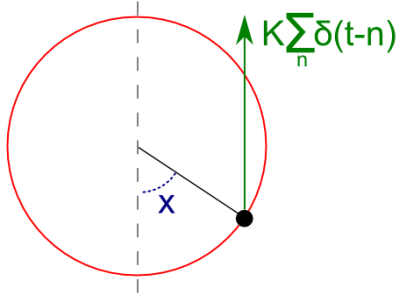
\includegraphics[width=0.33\textwidth]{kicked-rotor}

\begin{block}{Taylor, Chirikov and Greene  standard map}
\bea
x_{t+1} - x_{t} &=& p_{t+1} \qquad  \mod 1 \continue
p_{t+1} - p_{t} &=& F(x_{t})             \nnu
\eea
\end{block}

\medskip

\hfill $\to$ {\color{red}
chaos in Hamiltonian systems}
\end{frame} %%%%%%%%%%%%%%%%%%%%%%%%%%%%%%%%%%%%%%%%%%%%%%

\begin{frame}{the simplest example : a cat map evolving in time}

force
\(
 F(x) = Kx
\)
{\color{blue}linear} in the displacement $x$
\,,\;
$K\in\integers$
\bea
x_{t+1} &=& x_{t}+p_{t+1} \quad\;\;  \mod 1
        \continue
p_{t+1} &=& p_{t} + K x_{t} \qquad  \textcolor{red}{\mod 1}
\nnu
\eea
 \textcolor{red}{C}ontinuous
 \textcolor{red}{A}utomorphism of the
 \textcolor{red}{T}orus, or

\begin{block}{time-evolution cat map}
a linear, area preserving map of a 2-torus onto itself
 \[
 \left[\begin{array}{c}
   \ssp_{\zeit}  \\
   \ssp_{\zeit+1}
  \end{array} \right]=
  \jMps \left[\begin{array}{c}
   \ssp_{\zeit-1}  \\
   \ssp_{\zeit}
  \end{array} \right]
 - \left[\begin{array}{c}
 0  \\
 \Ssym{\zeit}
 \end{array} \right]
\,,\qquad
\jMps = \left[
\begin{array}{cc}
0 & 1 \\
-1 & s \\
\end{array}
    \right]
 \] %\ee{PerViv:2confRepMat}

\end{block}
for integer {\color{blue}`stretching' $s=\tr{\jMps} > 2$}
the map is \\ beloved by ergodicists :\\
hyperbolic $\Rightarrow$
{\color{blue}perfect chaotic Hamiltonian dynamical system}
\end{frame} %%%%%%%%%%%%%%%%%%%%%%%%%%%%%%%%%%%%%%%%%%%%%%

\begin{frame}{a cat is literally Hooke's wild, `anti-harmonic' sister}

\begin{block}{for $s<2$ Hooke rules}
local restoring oscillations

around the sleepy z-z-z-zzz resting state
\end{block}

\begin{block}{for $s>2$ cats rule}
exponential runaway

wrapped global around a \statesp\ torus
\end{block}
\bigskip

\hfill
{\color{red}cat} is to {\color{red}chaos}
what {\color{red}harmonic oscillator} is to {\color{red}order}
\vfill
\hfill
{\color{blue}there is no more fundamental example of chaos in mechanics}
\end{frame} %%%%%%%%%%%%%%%%%%%%%%%%%%%%%%%%%%%%%%%%%%%%%%

\renewcommand{\Xx}{\ensuremath{\Phi}}

\begin{frame}{(2) {\color{orange}spatio}{\templatt}}
\vfill
\begin{center}
{\huge lattice formulation}
% {\huge Lagrangian formulation}
\end{center}
\vfill
\end{frame} %%%%%%%%%%%%%%%%%%%%%%%%%%%%%%%%%%%%%%%%%%%%%%

\begin{frame}{cat map in lattice formulation}
replace momentum by velocity
\[
p_{t+1}=(\ssp_{t+1}  - \ssp_{t})/\Delta t
\]
obtain
 \[
 \left[\begin{array}{c}
   \ssp_{\zeit}  \\
   {\color{blue}\ssp_{\zeit+1}}
  \end{array} \right]=
  \left[
\begin{array}{cc}
0 & 1 \\
{\color{blue}-1} & {\color{blue}s} \\
\end{array}
    \right]
    \left[\begin{array}{c}
   {\color{blue}\ssp_{\zeit-1}}  \\
   {\color{blue}\ssp_{\zeit}}
  \end{array} \right]
 - \left[\begin{array}{c}
 0  \\
 {\color{blue}\Ssym{\zeit}}
 \end{array} \right]
 \] %\ee{PerViv:2confRepMat}

temporal lattice formulation % $(\ssp_{t},\ssp_{t-1})$
is {\Large pretty}\footfullcite{PerViv} :
\begin{block}{2-step difference equation}
\[
- \ssp_{t+1}  +  s \, \ssp_{t} - \ssp_{t-1} = \Ssym{t}
\] %\ee{eq:CatMapNewton1}
\end{block}
integer $\Ssym{t}$ ensures that

\hfill $\ssp_{t}$ lands in the unit interval

\bigskip
\[
\Ssym{t}\in  \A
\,,\quad \A\ = \{\mbox{finite alphabet}\}
\]
\end{frame} %%%%%%%%%%%%%%%%%%%%%%%%%%%%%%%%%%%%%%%%%%%%%%

\begin{frame}{think globally, act locally}

{\color{orange}spatio}{\templatt} at every instant $\zeit$,
{\color{blue}local} in time
\[
- \ssp_{t+1}  +  s \, \ssp_{t} - \ssp_{t-1} = \Ssym{t}
\] %\ee{eq:CatMapNewton1}
is enforced by the {\color{blue}global} equation
\beq
 \jMorb\,\Xx = \Mm
\,,
\ee{catTempLatt}
where
\end{frame} %%%%%%%%%%%%%%%%%%%%%%%%%%%%%%%%%%%%%%%%%%%%%%

\begin{frame}{orbit Jacobian matrix}
\[
 \jMorb\,\Xx - \Mm= 0
\]
with
\beq
{\Xx} % = \{\ssp_j\}
             = (\ssp_{\zeit+1},\cdots,\ssp_{\zeit+\cl{}})
\,,\quad
{\Mm} % = \{\Ssym{j}\}
             = (\Ssym{{\zeit+1}},\cdots,\Ssym{{\zeit+\cl{}}})
\ee{pathBern}
a
{\color{blue}{\lattstate}}, and a {\color{blue}symbol \brick}
\bigskip

and $[\cl{}\!\times\!\cl{}]$
 {\color{blue}\jacobianOrb} \jMorb\ is
\beq
- \shift{} + s\id - \shift{}^{-1}
=  \left(\begin{array}{ccccc}
    {s}   & -1    &      &         & -1\cr
    -1    & {s}   &-1    &         &   \cr
          & -1    &      & \ddots  &   \cr
          &       &      & {s}     &-1 \cr
    -1    &       &      & -1      & {s}
          \end{array} \right)
\ee{hopMatrix}
\end{frame} %%%%%%%%%%%%%%%%%%%%%%%%%%%%%%%%%%%%%%%%%%%%%%

\begin{frame}{think globally, act locally}
solving the {\color{orange}spatio}{\templatt} equation
\[
\jMorb\Xx=\Mm
\,,
\]
with
the $[\cl{}\!\times\!\cl{}]$ matrix ~~~~~
\(
\jMorb = -\shift{} + s\id - \shift{}^{-1}
\) %{tempBernFix}
\medskip

can be viewed as a search for zeros of the function
\beq
F[\Xx] = \jMorb\Xx-\Mm = 0
\ee{tempFixPoint}
where the entire {\color{blue}global lattice state} ${\Xx}_{\Mm}$ is
\medskip

a single {\color{blue}fixed point}
${\Xx}_{\Mm}=(\ssp_1,\ssp_{2},\cdots,\ssp_{\cl{}})$

\hfill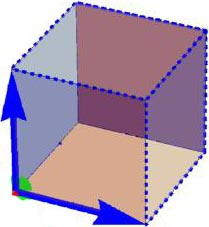
\includegraphics[width=0.12\textwidth]{hyperCube}

\hfill
in the \cl{}\dmn\ unit hyper-cube ~~~~~~~~~~~$\Xx\in[0,1)^\cl{}$
\end{frame} %%%%%%%%%%%%%%%%%%%%%%%%%%%%%%%%%%%%%%%%%%%%%%

\begin{frame}{fundamental fact in action}
% BernCyc2Jacob.svg
    \begin{block}{\templatt\  {\fundPip} for period 2}
square $[0BCD]$
$\Rightarrow\jMorb\,=\,$
{\fundPip} $[0B'C'D']$
\bigskip

\begin{center}
            \begin{minipage}[c]{0.32\textwidth}\begin{center}
% ChaosBook {fig:BernPartExam}
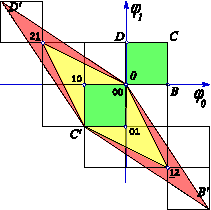
\includegraphics[width=1.0\textwidth]{catCyc2JacobUnit}
            \end{center}\end{minipage}
            \hspace{2ex}
            \begin{minipage}[c]{0.46\textwidth}
$N_2=|\Det\jMorb|=5$
\medskip

{\fundPip} \\
$=$  5 unit area quadrilaterals
            \end{minipage}
\end{center}
a periodic point per each unit volume
    \end{block}
\end{frame} %%%%%%%%%%%%%%%%%%%%%%%%%%%%%%%%%%%%%%%%%%%%%%

\begin{frame}{{\color{orange}spatio}{\templatt}  zeta function}
is the generating function that counts {\color{blue}orbits}
\medskip

substituting the {\color{blue}\HillDet} count of periodic lattice states
\[
N_n = \Det\jMorb
\]
into the
{topological} zeta func\-tion
\[
\zetatop(z)
  =   \exp \left(
    -\sum_{n=1} \frac{z^n}{n} N_n
    \right)
\]%\label{perOrbits:Isola90-13}
leads to the elegant explicit formula\footfullcite{Isola90}
\[
\zetatop(z)
 =  \frac{1 - s z + z^2}
         {1 - 2z + z^2}
\]%\label{perOrbits:Isola90-13}


\vfill\hfill
{\Huge \textcolor{red}{solved!}}
\end{frame} %%%%%%%%%%%%%%%%%%%%%%%%%%%%%%%%%%%%%%%%%%%%%%

\begin{frame}{a side remark to experts}
% BernCyc2Jacob.svg
    \begin{block}{slicing cats}
\begin{center}
            \begin{minipage}[c]{0.23\textwidth}\begin{center}
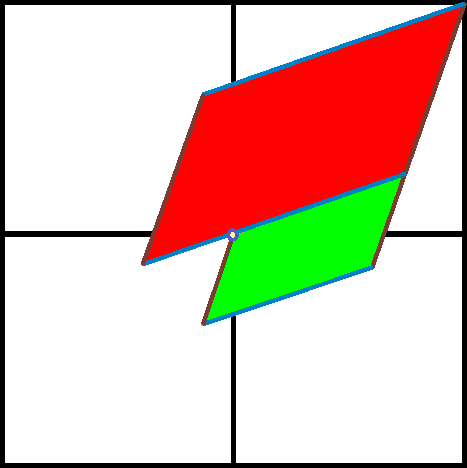
\includegraphics[width=1.0\textwidth]{PVAdlerWeissB-a}\\(a)
            \end{center}\end{minipage}
            \begin{minipage}[c]{0.23\textwidth}\begin{center}
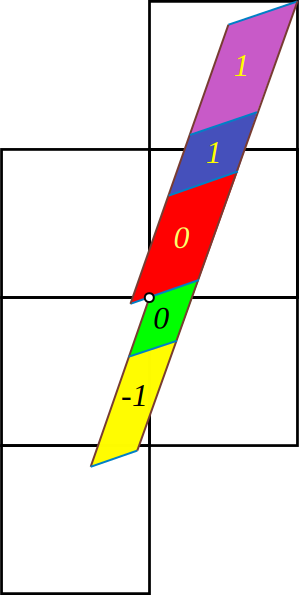
\includegraphics[width=1.0\textwidth]{PVAdlerWeissB-b}\\(b)
            \end{center}\end{minipage}
            \begin{minipage}[c]{0.23\textwidth}\begin{center}
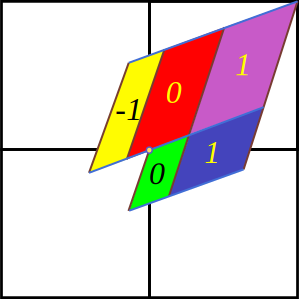
\includegraphics[width=1.0\textwidth]{PVAdlerWeissB-c}\\(c)
            \end{center}\end{minipage}
            ~~~
            \begin{minipage}[c]{0.12\textwidth}\begin{center}
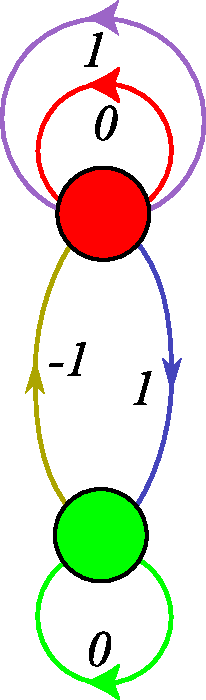
\includegraphics[width=1.0\textwidth]{PVAWMarkovCol}\\(d)
            \end{center}\end{minipage}
\end{center}

 is not the way
    \end{block}

\AW\ generating partition of the unit torus\\
is a distraction. Klein-Gordon is a deeper insight
\end{frame} %%%%%%%%%%%%%%%%%%%%%%%%%%%%%%%%%%%%%%%%%%%%%%

\begin{frame}{what continuum theory is \templatt\ discretization of?}
have
\begin{block}{2-step difference equation}
\[
- \ssp_{t+1} + s \, \ssp_{t} - \ssp_{t-1}
    =
\Ssym{t}
\] %\ee{eq:CatMapNewton1}
\end{block}
discrete lattice
\begin{block}{Laplacian in $1$ dimension}
\[
\ssp_{t+1} - 2\ssp_{t} + \ssp_{t-1}
     =
\Box\,\ssp_t
\]
\end{block}
\medskip

so \templatt\ is an (anti)oscillator chain, known as
\begin{block}{$d=1$ Klein-Gordon (or damped Poisson) equation (!)}
\[
 (-\Box + {\mu}^2)\,\ssp_{t} = \m_t
\,, \qquad
{\mu}^2= s-2
\] %\ee{LinearConn}
\end{block}
\vfill\hfill
\textcolor{red}{did you know that a cat map can be so cool?}
\end{frame} %%%%%%%%%%%%%%%%%%%%%%%%%%%%%%%%%%%%%%%%%%%%%%

\begin{frame}{a reminder slide, to skip : Helmholtz equation in continuum}
\begin{block}{inhomogeneous Helmoltz equation}
is an elliptical equation of form
\beq
   (\Box+k^2)\,\ssp(x)= -\Ssym{}(x)\,,\qquad x\in \reals^d
\label{CatMapContinuesPC}
\eeq
where $\ssp(x)$ is a $C^2$ function, and $\Ssym{}(x)$ is a function
with compact support
\end{block}

\bigskip

for the ${\mu}^2=-k^2>0$ (imaginary $k$), the equation is known as  the
{\color{blue}Klein-Gordon}, Yukawa, or
{\color{blue}screened Poisson equation}\footfullcite{FetWal03}
equation
\end{frame} %%%%%%%%%%%%%%%%%%%%%%%%%%%%%%%%%%%%%%%%%%%%%%

\begin{frame}{that's it! for spacetime of $1$ dimension}
lattice Klein-Gordon equation
    {\Huge
\[
  (-\Box + {\mu}^2)\,\ssp_{t} = \m_t
%    \,, \qquad
\] %\ee{LinearConn}
    }
\hfill solved completely and analytically!
\end{frame} %%%%%%%%%%%%%%%%%%%%%%%%%%%%%%%%%%%%%%%%%%%%%%


\begin{frame}{summary : think globally, act locally}
\bigskip
the problem of determining all global solutions stripped
to its bare essentials :
\bigskip
\begin{enumerate}
              \item
each solution a zero of the global {\color{blue}fixed point} condition
\[
F[\Xx] = 0
\]
              \item
compute  the {\jacobianOrb}
\[
\jMorb_{ij} =\frac{\delta F[\Xx]_i}{\delta \ssp_j}
\]
              \item
{\color{blue}fundamental fact} ~~~~~~~~
\(
N_\cl{} = |\Det\jMorb| =
\)
 period-$\cl{}$ states

 \bigskip
              \item
\hfill $\Rightarrow$ {\color{blue}zeta function} $\zetatop(z)$
            \end{enumerate}
\end{frame} %%%%%%%%%%%%%%%%%%%%%%%%%%%%%%%%%%%%%%%%%%%%%%

\section[\catlatt]
 {\catlatt}
\label{s:catLatt}



\end{document}
